\documentclass[a4paper, twocolumn, twoside]{article}
\usepackage{amsmath}
\usepackage{amssymb}
\usepackage[backend=biber]{biblatex}
\usepackage{hyperref}
\usepackage{xcolor}
\usepackage{minted}
\usepackage{tikz}
\usepackage{listofitems}
\usepackage{amsmath}
\usepackage{tcolorbox}
\usepackage{etoolbox}
\usepackage[
	top=2cm, % Top margin
	bottom=2cm, % Bottom margin
	left=1.5cm, % Left margin
	right=1.5cm, % Right margin
	footskip=1cm, % Space from the bottom margin to the baseline of the footer
	headsep=0.75cm, % Space from the top margin to the baseline of the header
	columnsep=20pt, % Space between text columns (in twocolumn mode)
]{geometry}

\addbibresource{references.bib}

\BeforeBeginEnvironment{minted}{\begin{tcolorbox}}%
\AfterEndEnvironment{minted}{\end{tcolorbox}}%

\colorlet{myred}{red!80!black}
\colorlet{myblue}{blue!80!black}
\colorlet{mygreen}{green!60!black}
\colorlet{myorange}{orange!70!red!60!black}
\colorlet{mydarkred}{red!30!black}
\colorlet{mydarkblue}{blue!40!black}
\colorlet{mydarkgreen}{green!30!black}

\tikzset{
  >=latex, % for default LaTeX arrow head
  node/.style={thick,circle,draw=myblue,minimum size=22,inner sep=0.5,outer sep=0.6},
  node in/.style={node,green!20!black,draw=mygreen!30!black,fill=mygreen!25},
  node hidden/.style={node,blue!20!black,draw=myblue!30!black,fill=myblue!20},
  node convol/.style={node,orange!20!black,draw=myorange!30!black,fill=myorange!20},
  node out/.style={node,red!20!black,draw=myred!30!black,fill=myred!20},
  connect/.style={thick,mydarkblue}, %,line cap=round
  connect arrow/.style={-{Latex[length=4,width=3.5]},thick,mydarkblue,shorten <=0.5,shorten >=1},
  node 1/.style={node in}, % node styles, numbered for easy mapping with \nstyle
  node 2/.style={node hidden},
  node 3/.style={node out}
}
\def\nstyle{int(\lay<\Nnodlen?min(2,\lay):3)} % map layer number onto 1, 2, or 3

\tikzstyle{densenode}=[thick,draw=blue,fill=blue!20,circle,minimum size=22]
\tikzstyle{activationnode}=[thick,draw=red,fill=red!20,circle,minimum size=22]

\hypersetup{
    colorlinks,
    linkcolor={black},
    citecolor={blue!50!black},
    urlcolor={blue!80!black},
	frenchlinks=true,
}

\title{Deep learning: Neural Network from scratch\\
\textit{creating a neural network library to solve the mnist dataset}}
\author{Adrien PELFRESNE - Alexis VAPAILLE}
\date{\today}


\begin{document}
	\onecolumn
    \maketitle
	\tableofcontents

	\twocolumn
	\section{Abstract}
	\textit{We have created a deep neural network library from scratch, in rust, without the use of any machine learning or deep learning library.\\
	The goal of this project was to solve the mnist dataset of handwritten digits and to provide a performance comparison between
	two multi-layer perceptrons, with and without convolution.\\
	Our library lets you create your sequential neural network, with a simple and declarative API and is widely open to extension.
	This project also includes a drawing mode, where you can draw your digit and see what each model guesses. The project is in a WIP stage, but we plan to improve it further shortly
	}

	\section{Motivation}
	Our motivation with this \textit{from scratch} approach was to deepen our understanding of neural networks.
	Because high-level libraries like \href{https://keras.io/}{Keras} and the incredible level of abstraction that comes with it,
	let us sometimes forget the inner machinery. Nevertheless,
	this underlying work that those libraries are doing is incredible, and we through it was a shame to be a simple user of those interfaces.\\
	The only (mathematical) helper library that we have used is \href{https://crates.io/crates/ndarray}{ndarray}
	which provides an n-dimensional container for general elements
	and numerics, as well as providing efficient matrix operations on the GPU.\\
	You can find our project on \href{https://github.com/dirdr/neural_network_from_scratch}{GitHub}, we widely encourage readers to check the source code,
	as in this report, we won't go into code-specific details and focus more on the abstract explanation.\\
	The workspace is split into multiple crates
	\begin{enumerate}
		\item The neural network library, under the crate \href{https://github.com/dirdr/neural_network_from_scratch/tree/main/nn_lib}{nn\_lib}
		\item The mnist example, which is using the \textit{nn\_lib} to define the networks and benchmark the dataset, Under the crate  \href{https://github.com/dirdr/neural_network_from_scratch/tree/main/mnist}{mnist}
		\item the GUI code to run an interactive drawing mode is included in the workspace in the app file.
            \item this \href{https://github.com/dirdr/neural_network_from_scratch/tree/main/report}{report} source code
	\end{enumerate}

	\section{Sequential neural network}
	The multi-layer perceptron is known  as a \textit{Sequential} neural network, meaning that the \textbf{output}
	$Y_N$ of the layer $L_N$ is the \textbf{input} $X_{N+1}$ of the next layer $L_{N+1}$.\\
	$$
	Y_{N} = X_{N+1}
	$$
	and conversely,
	$$
	X_{N} = Y_{N-1}
	$$
	with subscript $N$ identifying layers in sequential order.
	from the input layer, when we pass our data,
	through the output layer, data flows in the network, passing
	through different kinds of layers.

      \begin{figure}
      \centering
        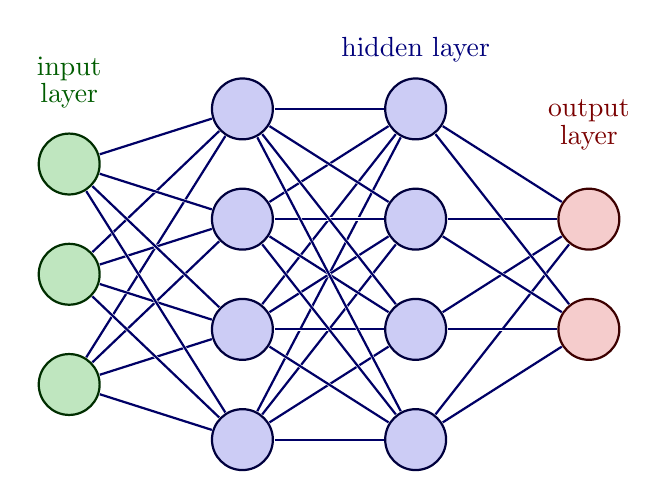
\begin{tikzpicture}[x=2.2cm,y=1.4cm]
            \message{^^JNeural network without text}
            \readlist\Nnod{3,4,4,2}
            \message{^^J  Layer}
            \foreachitem \N \in \Nnod{
            \def\lay{\Ncnt}
            \pgfmathsetmacro\prev{int(\Ncnt-1)}
            \message{\lay,}
            \foreach \i [evaluate={\y=\N/2-\i; \x=\lay; \n=\nstyle;}] in {1,...,\N} {         
              \node[node \n] (N\lay-\i) at (\x,\y) {};          
              \ifnum\lay>1
                \foreach \j in {1,...,\Nnod[\prev]}{ 
                  \draw[connect,white,line width=1.2] (N\prev-\j) -- (N\lay-\i);
                  \draw[connect] (N\prev-\j) -- (N\lay-\i);
                }
              \fi 
            }
        }
        \node[above=5,align=center,mygreen!60!black] at (N1-1.90) {input\\[-0.2em]layer};
        \node[above=2,align=center,myblue!60!black] at (N3-1.90) {hidden layer};
        \node[above=10,align=center,myred!60!black] at (N\Nnodlen-1.90) {output\\[-0.2em]layer};
        
        \end{tikzpicture}
        \caption{Visual representation of a sequential neural network}
    \end{figure}

	\subsection{General layer interface}
	We have defined a general \textit{Layer} interface, to be implemented by all the different layers we're going to use.\\
	This interface has two main method : \textbf{feed\_forward} and \textbf{propagate\_backward},
	The \textit{feed forward} method takes the input vector $X \in \mathbb{R}^i$ as a parameter and returns the output vector $Y \in \mathbb{R}^j$ of the layer.
	The \textit{propagate backward} method take as parameters the layer output gradient $\frac{\partial C}{\partial Y}$ and return the layer input gradient $\frac{\partial C}{\partial X}$.
	We will cover the use of these functions later, alongside the theoretical explanation of those concepts.

	\subsection{Dense layer}
	A dense layer, also known as \textit{Linear layer}, is a layer where each input neuron is connected to every output neuron,
	each connection is called a \textit{weight}. $w_{ij}$ is the weight
	connecting neuron $x_i$ (input) to neuron $y_j$ (output).

	\begin{figure}[H]
		\centering
		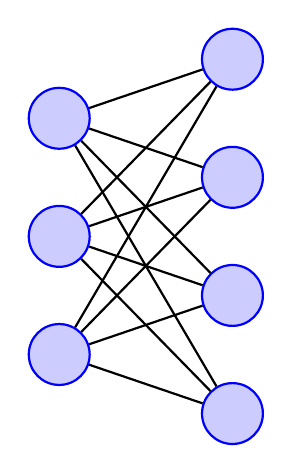
\begin{tikzpicture}[x=2.2cm,y=1.5cm]
		  \readlist\Nnod{3,4} % number of nodes per layer
		  % \Nnodlen = length of \Nnod (i.e. total number of layers)
		  % \Nnod[1] = element (number of nodes) at index 1
		  \foreachitem \N \in \Nnod{ % loop over layers
			% \N     = current element in this iteration (i.e. number of nodes for this layer)
			% \Ncnt  = index of the current layer in this iteration
			\foreach \i [evaluate={\x=\Ncnt; \y=\N/2-\i+0.5; \prev=int(\Ncnt-1);}] in {1,...,\N}{ % loop over nodes
			  \node[densenode] (N\Ncnt-\i) at (\x,\y) {};
			  \ifnum\Ncnt>1 % connect to the previous layer
				\foreach \j in {1,...,\Nnod[\prev]}{ % loop over nodes in previous layer
				  \draw[thick] (N\prev-\j) -- (N\Ncnt-\i); % connect arrows directly
				}
			  \fi % else: nothing to connect the first layer
			}
		  }
		\end{tikzpicture}
	\caption{Dense Layer with 3 input nodes and 4 output nodes}
	\end{figure}
	
	We calculate a dense layer neuron output value $y_j$ as 
	$$
	y_j = \sum_{i=1}^{n} x_i w_{i,j} + b_j
	$$

	which is the bias-corrected weighted sum of all the connected input nodes.
	$b_j$ is the bias term for the output neuron $j$.
	We can rewrite this operation to use matrix operation on whole vectors.

	$$
	Y = XW + B
	$$

	with $Y \in \mathbb{R}^j$, $X \in \mathbb{R}^i$, $W \in M_{i*j}(\mathbb{R})$ and $B \in \mathbb{R}^j$\\
	In this report, we will annotate vectors : $X \in \mathbb{R}^N$, but note that to
	be able to do the matmul in practice, a vector will be broadcasted to a matrix $M_{1*i} (\mathbb{R})$

	\subsection{Activation layer}

        Activation functions introduce non-linearity into the neural network. Without them, the network would be a series of linear transformations, regardless of the number of layers, making it equivalent to a single-layer model. Non-linear activation functions allow the network to learn
        to separate data in a non-linear way
 
	There are two schools of thought for defining activations.
	\begin{enumerate}
		\item activations are used to produce the \textbf{output value inside} a dense layer,
			in this case, the weighted sum of the dense layer is called $z$, and $y$ is calculated by applying
			an activation $\sigma$ to $z$ : $y : \sigma(z)$.
		\item activations are used \textbf{outside} the dense layer  in this case,
			the output of a dense layer $y$ is equal to the weighted sum $z$.
			An activation layer is placed just after the dense layer,
			 applying the activation function to each neuron.
	\end{enumerate}

	We implemented our sequential neural network with the second paradigm,
	because it is easier in code to manage a dense and an activation layer separately, mainly for backpropagation calculation ease.

	\begin{figure}[H]
	\centering
	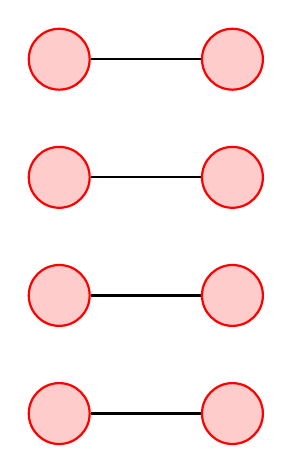
\begin{tikzpicture}[x=2.2cm,y=1.5cm]
	  \readlist\Nnod{4,4} % Define two layers, each with 4 nodes
	  % Loop over both layers
	  \foreachitem \N \in \Nnod{
		\foreach \i [evaluate={\x=\Ncnt; \y=\N/2-\i+0.5; \prev=int(\Ncnt-1);}] in {1,...,\N}{
		  \node[activationnode] (N\Ncnt-\i) at (\x,\y) {};
		  % If not the first layer, connect nodes from the previous layer
		  \ifnum\Ncnt>1
			\draw[thick] (N\prev-\i) -- (N\Ncnt-\i); % Connect nodes element-wise
		  \fi
		}
	  }
	\end{tikzpicture}
	\caption{Activation layer with 4 input neuron}
	\end{figure}

	The Activation layer takes a vector $X \in \mathbb{R}^n$  as input and produces a vector $Y \in \mathbb{R}^n $ as output,
	with the activation function applied to each neuron.\\
	We must note that some activations function transform a vector by
	mapping the vector individual components $x$ through the function, like ReLU

	$$
	ReLU(x) = max(0, x)
	$$

	While other activation functions, like \textit{softmax} work on whole vectors.
	Softmax takes a vector $z \in \mathbb{R}^K$,
	and converts it into a probability distribution of $K$ possible outcomes.

	$$
	\sigma : \mathbb{R}^{K} \rightarrow (0, 1)^K, K \geq 1
	$$

	is computed by taking a vector $z = (z_1, ..., z_k) \in \mathbb{R}^K$ and compute each component of a vector $\sigma(\mathbf{z}) \in (0, 1)^K$ 

	$$
	\sigma(\mathbf{z})_i = \frac{e^{z_i}}{\sum_{j = 1}^{K} e^{z_j}}
	$$

	Current activations functions implemented in our library are :
	\begin{itemize}
		\item{Sigmoid}
		\item{ReLU}
		\item{Tanh}
		\item{Softmax}
	\end{itemize}

	\section{Cost function}
	To measure how well a neural network performs, we use a cost function, 
	which outputs a real number
	by comparing the neural network \textit{output}, 
	and the \textit{observed} value. For the mnist dataset, the \textit{output} value is what the neural network guesses for the image we feed him with, and the \textit{observed} value is the real label for that image (the digit the image is).\\
	A simple cost function is the mean-squared error :
	$$
	\text{MSE} = \frac{1}{n} \sum_{i=1}^{n} (\hat{y}_i - y_i)^2
	$$
	The MSE function is great for regression neural networks when we want to predict a continuous value from an input.\\
	To do classification, like in the mnist data of handwritten digits,
	we use another cost function :
	the cross entropy cost function
	$$
		\text{Cross Entropy} = -\sum_{c=1}^{C} y_{c} \log(\hat{y}_{c})
	$$
	with $C$ the number of classes (e.g, 10 for the mnist dataset), $y_{c}$ 
	the observed probability, and $\hat{y}_{c}$ the neural network output.\\
	This expression simplifies to

	$$
		\text{Cross Entropy} = -\log(\hat{y}_{c})
	$$

	if $y_{c}$ is one hot encoded (i.e, 1 for the observed class and 0 for others).

	\section{The learning process}
	\subsection{Gradient}
	The gradient of a function $\nabla f$ is the vector field that represents the direction
	and rate of the quickest increase of the function from a point $p$.\\
	We can visualize the gradient and the curve of a function $f(x, y) = -(\cos^2 x  +\cos^2 y)^2$\\

	\begin{figure}[H]
		\begin{center}
			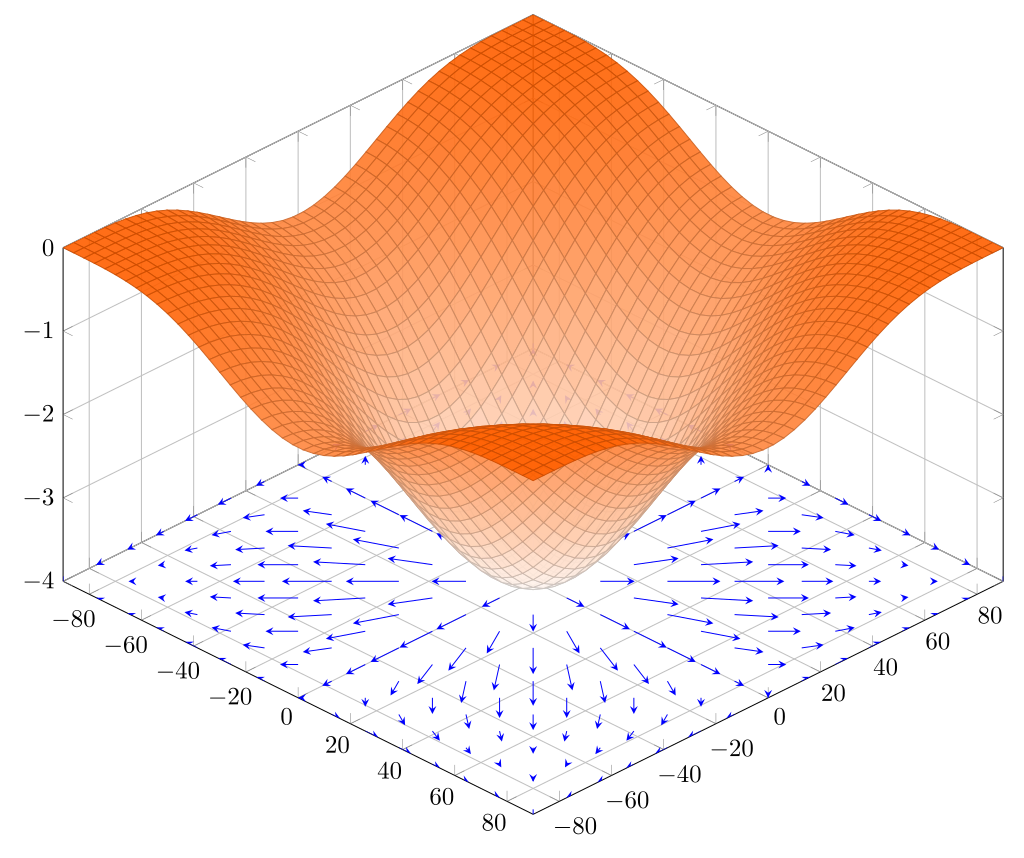
\includegraphics[width=\columnwidth]{images/gradient_2d.png}
		\end{center}
		\caption{Function representation and gradient field of the function $-(\cos^2 x  +\cos^2 y)^2$}\label{fig:gradien2d}
	\end{figure}

	The field vector below the function curve represents the gradient,
	for each point $p = (x, y)$ the arrow at $p$ point toward the direction
	with the fastest increase of $f$.
        This is useful in optimization problems when we want to find the maximum or the minimum
        of the function, because it indicates to us which direction to follow at a certain point,
        to maximize, or minimize the value of the function.

	\subsection{Minimization}
	To make our neural network lean, we adjust its parameters (i.e, weights and biases for a dense layer)
	to \textbf{minimize the cost function $C$ of the network}.
	We can use the cost function gradient, which tells us the direction and magnitude
	of the fastest \textbf{increase} of cost, and proceed to go in the opposite direction,
	which will make us go toward the fastest \textbf{decrease} of the cost function.\\
	The algorithm used to minimize the cost function is the \textit{gradient descent},
	which will repeatedly descend the curve by going toward the opposite of the gradient of the cost function.

	Here is the process for a single gradient descent step :
	\begin{enumerate}
		\item feeds all input data points into the network,
			calculating the cost for every output.
		\item calculates the average cost.
		\item computes the gradient of the averaged cost function \textbf{with respect to the network parameters}.
		\item update the parameters in the opposite direction of the gradient
	\end{enumerate}

	\subsection{backpropagation}
	To do a gradient descent step, we need the gradient of
	the cost function with respect to the neural network parameters $\frac{\partial C}{\partial P}$
	the algorithm used to calculate this gradient 
	is called \textbf{backpropagation}.\\
	Backpropagation precisely calculate
	(and not only estimate like the finite difference method) the gradient of the cost function $C$ with respect to the neural network parameters,
	which we will call parameters gradient $\frac{\partial C}{\partial P}$.\\
	The key mathematical tool used in backpropagation is the chain rule,
	which allows the gradient of the cost function
	to be split into a gradient of simpler functions at each neuron within the network.\\
	For each layer, $L_n$, to calculate the parameter's gradient $\frac{\partial C}{\partial P_n}$,
	we need to know the output gradient $\frac{\partial C}{\partial Y_n}$, this gradient is given to us by the next layer in the sequential order,
	because in the sequential architecture $\frac{\partial C}{\partial X_{n+1}} = \frac{\partial C}{\partial Y_n}$.
	We want to also calculate $\frac{\partial C}{\partial X_i}$, the input $X$ gradient,
	to transmit it to the previous layer, which needs it to calculate her own parameters gradient $\frac{\partial C}{\partial P_{i-1}}$.\\
	You can probably feel why this process is called backpropagation, we are sharing gradients,
	from layer to layer, starting at the last layer and going back up to the start of the net.\\
	Each layer will have her implementation of \textbf{propagate backward method},
	in the next sections, we will cover the calculation for the layer we used in our library.

	\subsection{Dense layer backpropagation}

	The dense layer has two trainable parameters, the weights $W$, and the biases $B$.
	Starting with the gradient of the cost function with respect to the weights, we are given
	the output gradient :
	\begin{align}
		\frac{\partial C}{\partial Y} &= \begin{bmatrix}
		\frac{\partial C}{\partial y_1} \\
		\frac{\partial C}{\partial y_2} \\
        \vdots \\
	   \frac{\partial C}{\partial y_j} \\
	\end{bmatrix}
	\end{align}
	The cost function $C$ depends on $Y$ which depend on $W$ thus $C$ depend on $W$ (chain rule)
	$$
    \frac{\partial C}{\partial W} = \frac{\partial C}{\partial Y} \frac{\partial Y}{\partial W}
	$$
	We calculate each weight gradient component $\frac{\partial C }{\partial W_{ij}}$
	$$
    \frac{\partial C}{\partial W_{ij}} = \sum_{l=1}^{N} \frac{\partial L}{\partial Y_{lj}} \frac{\partial Y_{lj}}{\partial W_{ij}}
	$$
	because $W_{ij}$ is used in every example for calculating the $j^{th}$ column of the output matrix. Let's look at the formula for $Y_{lj}$ to get the derivative
	$$
		Y_{lj} = X_{l1}W_{1j} + \cdots + X_{li}W_{ij} + \cdots + X_{lp}W_{pj} + b_{j}
	$$
	$$
		\frac{\partial Y_{lj}}{\partial W_{ij}} = X_{li}
	$$
	$$
		\implies \frac{\partial C}{\partial W_{ij}} = \sum_{l=1}^{N} \frac{\partial C}{\partial Y_{lj}} X_{li} = \sum_{l=1}^{N} X^{T}_{il}\frac{\partial C}{\partial Y_{lj}}
	$$
	So finally 
	$$
		\frac{\partial C}{\partial W} = X^{T} \frac{\partial C}{dY}
	$$
	for the biases $B$.
	\begin{align}
		\frac{\partial C}{\partial b} &= \frac{\partial C}{\partial Y} \frac{\partial Y}{\partial b}\\
		\frac{\partial C}{\partial b_{i}} &= \sum_{l=1}^{N} \frac{\partial C}{\partial Y_{li}} \frac{\partial Y_{li}}{db}
	\end{align}
	since the bias term $b_{i}$ is used in the evaluation of the entire column of $Y$.
	$$
		\frac{\partial Y_{li}}{\partial b_{i}} = 1
	$$
	$$
		\frac{\partial C}{db_{i}} = \sum_{l=1}^{N} \frac{\partial C}{\partial Y_{li}}
	$$
	$$
		\frac{\partial C}{\partial b} = \frac{\partial C}{\partial Y}
	$$
	and lastly, we calculate the gradient with respect to $X$
	\begin{align}
		\frac{\partial C}{\partial X} &= \frac{\partial C}{\partial Y} \frac{\partial Y}{\partial X}\\
		\frac{\partial C}{\partial X_{ij}} &= \sum_{l=1}^{k} \frac{\partial C}{\partial Y_{il}} \frac{\partial Y_{il}}{\partial X_{ij}}
	\end{align}
	since the data point $i$ will only influence the data point $i$ in $Y$. Other data points will not be affected. Further, $X_{ij}$ is used in the calculation of every dimension of $Y_{i,:}$. To calculate the gradient,

	$$
		Y_{il} = \sum_{t=1}^{p} X_{it}W_{tl}
	$$
	$$
		\frac{\partial Y_{il}}{\partial X_{ij}} = W_{jl}
	$$
	$$
		\frac{\partial C}{\partial X_{ij}} = \sum_{l=1}^{k} \frac{\partial C}{\partial Y_{il}}W_{jl}
		= \sum_{l=1}^{k} \frac{\partial C}{\partial Y_{il}} W_{lj}^{T}
	$$
	$$
		\implies \frac{\partial C}{\partial X} = \frac{\partial C}{\partial Y} W^{T}
	$$
	\subsection{Activation layer backpropagation}
	An activation layer doesn't have any trainable parameters, We just need to calculate the input gradient.\\
	We are given
	the output gradient $\frac{\partial C}{\partial Y}$,
	we know that 

	\begin{align*}
		Y &= \begin{bmatrix}
		f(X_1) \\
		f(X_2) \\
        \vdots \\
		f(X_i)
	\end{bmatrix}
	\end{align*}
        applying the chain rule like before,
	$$
    \frac{\partial C}{\partial X} = \frac{\partial C}{\partial Y} \frac{\partial Y}{\partial X}
	$$
        calculating each component
	$$
    \frac{\partial C}{\partial X_{ij}} = \sum_{l=1}^{N} \frac{\partial C}{\partial Y_{lj}} \frac{\partial Y_{lj}}{\partial X_{ij}}
	$$

	using the same procedure as for the previous calculations

	$$
	\implies \frac{\partial C}{\partial X} = \frac{\partial C}{\partial Y} \odot Y\prime
	$$

	with 

	\begin{align*}
		Y\prime &= \begin{bmatrix}
		f\prime(X_1) \\
		f\prime(X_2) \\
        \vdots \\
		f\prime(X_i)
	\end{bmatrix}
	\end{align*}

	\section{Optimizers}
	
	To update a neural network parameter $\theta$, we use the gradient descent formula,
	with a fixed learning rate $\eta$

	$$
	\theta := \theta - \eta \frac{\partial C}{\partial \theta}
	$$

        Updating the neural network layers parameters with this method  is known, in the Keras API, as the \textit{Stochastic gradient descent optimizer},
	but other ways of updating layer parameters exist, we call those alternative methods \textbf{optimizers}. One of the best ones is Adam \cite{kingma2017adam}

	\subsection{Adam}
	Adam accelerates the convergence towards the optimal set of parameters by taking into account past gradient,
	it will also adapt the learning rate for each parameter.

	ADAM initializes two vectors, 
	$m$ and $v$, which store the exponential moving averages of past gradients and past squared gradients,
	respectively. These vectors are used to scale the gradient updates adaptively.

	\begin{enumerate}
	  \item \textbf{Initialization:} Initialize two vectors, $m$ and $v$, to store the moving averages of the gradients and their squares, respectively.
	  \item \textbf{Computing Moving Averages of the Gradients:}
		\begin{align*}
		  m_t &= \beta_1 \cdot m_{t-1} + (1 - \beta_1) \cdot g_t, \\
		  v_t &= \beta_2 \cdot v_{t-1} + (1 - \beta_2) \cdot g_t^2,
		\end{align*}
		where $g_t$ is the gradient at time step $t$, and $\beta_1$ and $\beta_2$ are factors that control the decay rates.
	  \item \textbf{Bias Correction:} Correct initial bias in $m$ and $v$:
		\begin{align*}
		  \hat{m}_t &= \frac{m_t}{1 - \beta_1^t}, \\
		  \hat{v}_t &= \frac{v_t}{1 - \beta_2^t}.
		\end{align*}
	  \item \textbf{Update Weights:} Adjust weights based on the corrected moments:
		\begin{equation*}
		  \theta_{t+1} = \theta_t - \frac{\eta}{\sqrt{\hat{v}_t} + \epsilon} \cdot \hat{m}_t,
		\end{equation*}
		where $\theta$ are the parameters, $\eta$ is the learning rate, and $\epsilon$ is a small constant for numerical stability.
	\end{enumerate}

	\section{Batching}
	We went through several feed-forward implementations in our code. The first one was to pass data points $x \in \mathbb{R}^{i}$ one by one, in the network.
    This was very slow, for example, for the mnist dataset, which has 60k training examples,
	we were going through the whole neural network: feed forward, cost evaluation, and back-propagation 60k times.\\
	We then learned that we can adapt our code to pass \textit{a batch} of data to the neural network, this batch can be of any length.
	The input then becomes, $x \in M_{n*i} (\mathbb{R})$ with each line of the input matrix representing a single data point.
	The calculation became much faster because we can now feed $n$ element at a time in the neural network.

	\section{Initializer}
	Initializers determine the starting weights of a neural network, it is important to choose the right initializer, depending on our network architecture, to avoid problems like vanishing or exploding gradients, and to optimize convergence.
	At the moment, we are writing this report, we have implemented two initializers inside our library,

	\begin{enumerate}
		\item{he}
	The \textit{He} initializer, designed for \textit{ReLu} activation functions,
	initializes weights from a normal distribution centered at zero with a standard deviation of 
	$\sqrt{\frac{2}{n}}$ (where $n$ is the number of input nodes).
	This setup helps prevent the vanishing gradient problem in deep networks with \textit{ReLu} activations,
	ensuring that gradients remain large enough to sustain effective learning through many layers.
		\item
	Conversely, the \textit{Glorot Uniform} initializer, 
	also known as Xavier Uniform, is ideal for networks using \textit{sigmoid} or \textit{Tanh} activations.
	It selects weights from a uniform distribution within $[-c, c]$,
	where $c = \sqrt{\frac{6}{n_{\text{in}} + n_{\text{out}}}}$.
	This approach maintains a balance in the variance of neurons' outputs across the network,
	aiding in stable gradient flow in deep networks with saturating activations.
	\end{enumerate}

	\section{Convolutional neural network}
	ALEXIS a toi de travailler

	\section{Metrics}
	The mnist dataset, is a classification problem, we can implement multiple metrics
	to evaluate the network performances, we will explain the one we implemented in our library.

	\begin{enumerate}
		\item Accuracy measures the proportion of correct prediction to the total observations in the dataset.
		for example, if we have correctly classified 950 images out of 1000, the accuracy will be 95 percent.
		$$
		\text{Accuracy} = \frac{\text{Number of Correct Predictions}}{\text{Total Number of Predictions}}
		$$

		Precision and Recall are two metrics acting on a specified class.
		\textbf{Retrieved elements} are all the network predictions for a specific class.
		\textbf{Relevant elements} are all the correct instances of 
		the class \cite{wiki_precision_recall}.

		\item Precision answer the question : \textit{How many retrieved items are relevant}
		$$
		\text{Precision} = \frac{\text{Relevant retreived instance}}{\text{All retrieved instance}}
		$$
		\item Recall answers the question: \textit{How many relevant items are retrieved}
		$$
		\text{Recall} = \frac{\text{Relevant instances}}{\text{All relevants instance}}
		$$
	\end{enumerate}

        Those metrics are important to evaluate the network performances, in our implementations and results analysis, we focused on cost and accuracy, but recall, precision, and other classification metrics
        can be useful to know on which specific digits the neural network is making mistakes.

	\section{Training, Validation, and Test Sets}
	To monitor the performances of a neural network effectively,
	it is important to break down the dataset into three distinct subsets:
	training, validation, and test sets.

	\begin{itemize}
        \item{\textbf{Training set}}: Is used during the learning phase,
        with training data directly influencing the parameter updates
        \item{\textbf{Validation set}}: Is used to provide an unbiased evaluation of a model fit
        on the training dataset while tuning the model's hyperparameters.
        This set is used during training, to prevent overfitting when the model performs well on the training data
        but poorly on unseen data.
        \item{\textbf{Test set}}: Is used only after the model's training and validation phases are complete.
	It provides the final, unbiased performance metric of the neural network.
	\end{itemize}

	\section{Results}
    \subsection{Network declaration}
	We include a small code snippet, showing our custom library API to declare a sequential neural network. You can find the API for a sequential network declaration inside the \href{https://github.com/dirdr/neural_network_from_scratch/blob/main/nn_lib/src/sequential.rs}{sequential module}, and the declaration of the mnist network in the \href{https://github.com/dirdr/neural_network_from_scratch/blob/main/mnist/src/network_definition.rs}{network declaration module}

	\begin{minted}[breaklines, tabsize=2]{rust}
let net = NeuralNetworkBuilder::new()
	.push(DenseLayer::new(
		784,
		32,
		InitializerType::He,
	))
	.push(
		ActivationLayer::from(Activation::ReLU)
	)
	.push(
		DenseLayer::new(32, 10, InitializerType::He)
	)
	.push(
		ActivationLayer::from(
			Activation::Softmax
		)
	);
	.watch(MetricsType::Accuracy)
Ok(net.compile(GradientDescent::new(0.01), CostFunction::CrossEntropy)?)
	\end{minted}

	The layers are added in sequential order with the push method.
	the \textit{watch} method will add a \textit{MetricsType} to the list of metrics that the program needs to calculate, in the example we watched the accuracy metrics.
	those metrics are given by epochs for the training and validation dataset. and at the end of the test dataset.

    \subsection{Vapnik–Chervonenkis tradeoff}

	To create a great network, we will try to reach the \textit{VC trade-off principle} \cite{LeCun2019} \cite{vapnik1974theory},
	this principle states that:

	\begin{enumerate}
		\item A more complex model might fit the training data very well (low training error)
			but risks overfitting, meaning it could perform poorly on new data
			because it is too tailored to the training set (high variance).
		\item A less complex model might not fit the training data as closely 
			(higher training error) but can generalize better on new data because 
			it does not capture the noise and specific details of the training set (low variance).
	\end{enumerate}

	Our challenge will thus be, to find the right level of complexity that minimizes both the error on the training data.

	\subsection{Multi-layer perceptron}
        \subsubsection{Overfitting}
	   We will analyze the result of an overfitting model, to see 
	how this behavior translates into metrics. To make a model overfit, we have multiple options

	\begin{itemize}
		\item increase the model complexity (number of hidden layers, number of neurons per layer)
		\item reduce the batch size to make the learning process very granular 
			and increase the chance of the network learning too many specific patterns
	\end{itemize}

	In our case we have chosen to lower the batch size, here are our network hyperparameters

	\begin{table}[H]
	\centering
	\begin{tabular}{|l|c|c|}
	\hline
	hyperparameters & epochs & batch size  \\
	\hline
	Value & 30 & 5   \\
	\hline
	\end{tabular}
	\caption{hyperparameters overfitting model}
	\end{table}
        Here is the cost comparison, over 30 epochs between the training cost, and the validation cost.
	\begin{figure}[H]
		\begin{center}
			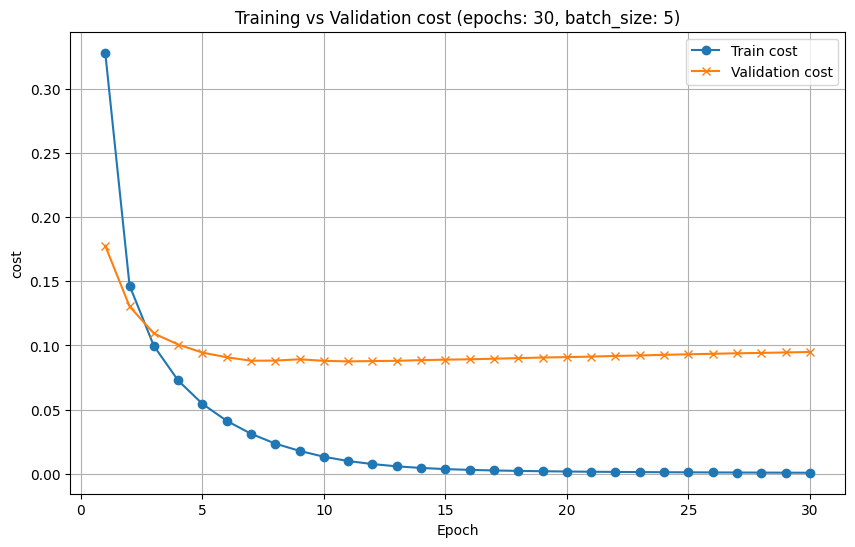
\includegraphics[width=\columnwidth]{images/cost_overfit.png}
		\end{center}
		\caption{Training vs. Validation cost overfitting model}\label{fig:cost_overfit}
	\end{figure}

	The overfitting stands out, our train cost gets very low, while the validation cost remains stable
	this means that our neural network has learned too many specific patterns in the training data,
	making the error go very low on this set, but on the validation set, the network
	doesn't generalize well

	\begin{figure}[H]
		\begin{center}
			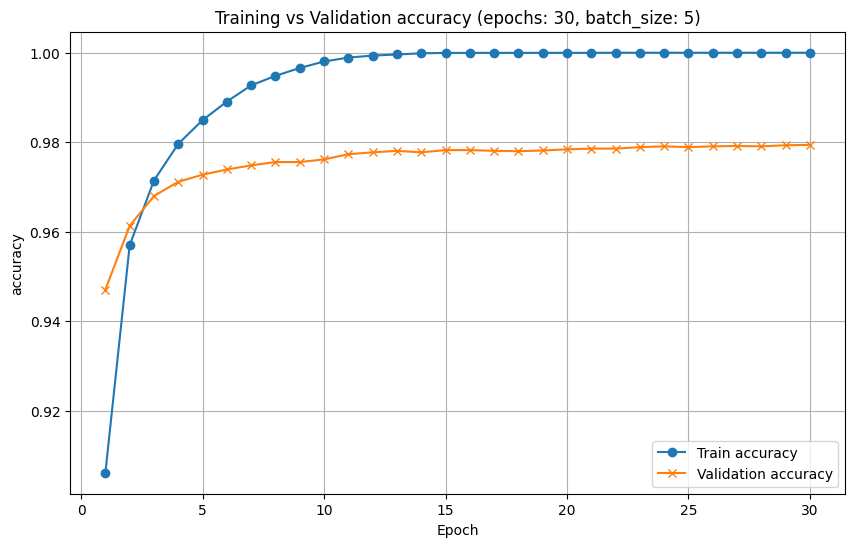
\includegraphics[width=\columnwidth]{images/accuracy_overfit.png}
		\end{center}
		\caption{Training vs. Validation cost overfitting model}\label{fig:accuracy_overfit}
	\end{figure}

	The same observation applies to the evolution of accuracy over epochs.
	Accuracy reached a stunning 100 percent on our training data, meaning that it doesn't make any mistakes, but the validation accuracy struggles to get over 98 percent.\\

        \subsubsection{Greatfitting}
	We have achieved our best generalization with the following hyperparameters and network definitions.
	\begin{table}[H]
	\centering
	\begin{tabular}{|l|c|c|}
	\hline
	hyperparameters & epochs & batch size  \\
	\hline
	Value & 15 & 100   \\
	\hline
	\end{tabular}
	\caption{hyperparameters great fitting model}
	\end{table}


	\begin{minted}[breaklines, tabsize=2]{rust}
let net = SequentialBuilder::new()
	.push(
		DenseLayer::new(784, 256,
		InitializerType::He))
	.push(
		ActivationLayer::from(
			Activation::ReLU)
		)
	.push(
		DenseLayer::new(256, 256,
		InitializerType::He))
	.push(
		ActivationLayer::from(
			Activation::ReLU)
		)
	.push(
		DenseLayer::new(256, 10,
		InitializerType::GlorotUniform))
	.push(
		ActivationLayer::from
		(
			Activation::Softmax)
		)
	.watch(MetricsType::Accuracy);
Ok(net.compile(GradientDescent::new(0.04), CostFunction::CrossEntropy)?)
	\end{minted}
        Here is the comparison between the training cost and the validation cost :
	\begin{figure}[H]
		\begin{center}
			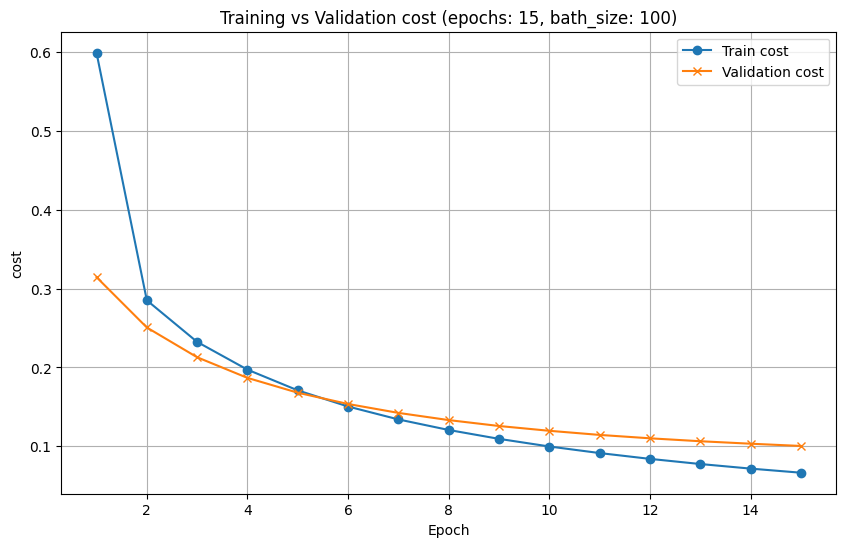
\includegraphics[width=\columnwidth]{images/cost_greatfit.png}
		\end{center}
		\caption{Training vs. Validation cost great fitting model}\label{fig:cost_greatfit}
	\end{figure}
	Here, our model seems to have generalized patterns, because the training cost and 
	the validation cost follows the same path, slowly increasing, with the gap between curves never blowing off the roof.
	We reach a validation cost of 0.097, and the cost for the testing data set is 0.091.
	\begin{figure}[H]
		\begin{center}
			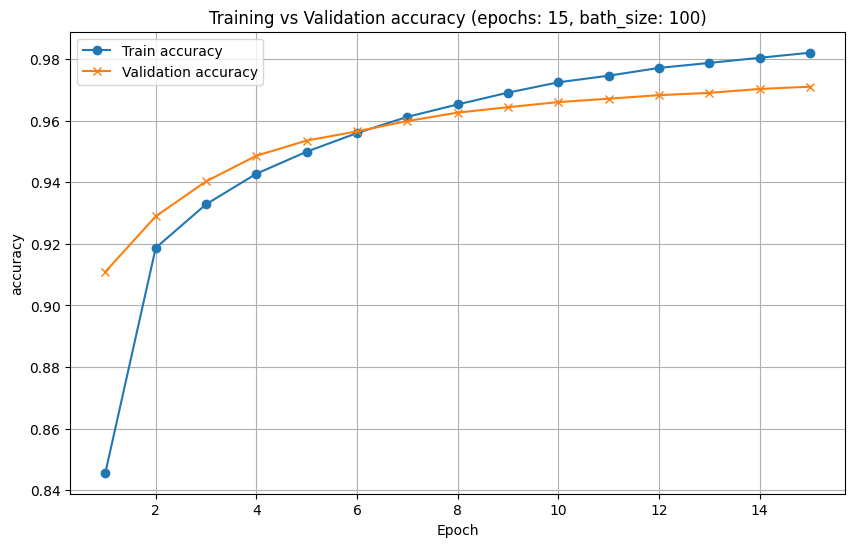
\includegraphics[width=\columnwidth]{images/accuracy_greatfit.png}
		\end{center}
		\caption{Training vs. Validation cost great fitting model}\label{fig:accuracy_greatfit}
	\end{figure}
	We reach a validation accuracy of 97.10 percent for the final epochs, and the accuracy for the testing data set is 97.31 percent.
	which is not a \textit{state-of-the-art} accuracy, but is a good result.
	\subsection{Convolutional multi-layer perceptron}
        Alexou fais les resultats !!
	\section{Conclusion}
	This project of creating our own \textit{from scratch} library has brought us a lot of knowledge,
	It has made us greatly understand the whole neural network process.
	We have planned to add more functionality to our library and optimize the code base even after the end of this project.
	We want to add more optimizers, the dropout layer, and a learning rate scheduler.
	and over the longer term, we'd like to add other neural network paradigms, such as Recurrent neural networks, and use our library for our experiments with deep learning!
	\nocite{*}
	\printbibliography
\end{document}

